\section{Results}
\label{sec:results}

\TODO{Introduce}


\subsection{Repo-level analysis}
\label{sec:results1}

\TODO{Graphics placement}

This subsection focuses solely on repository-level analysis of our metrics, since comparison between individual commits and or individual authors would be tedious. Also, author-level analysis is open to everyone through the web interface.

\begin{figure}[p]
    \centering
    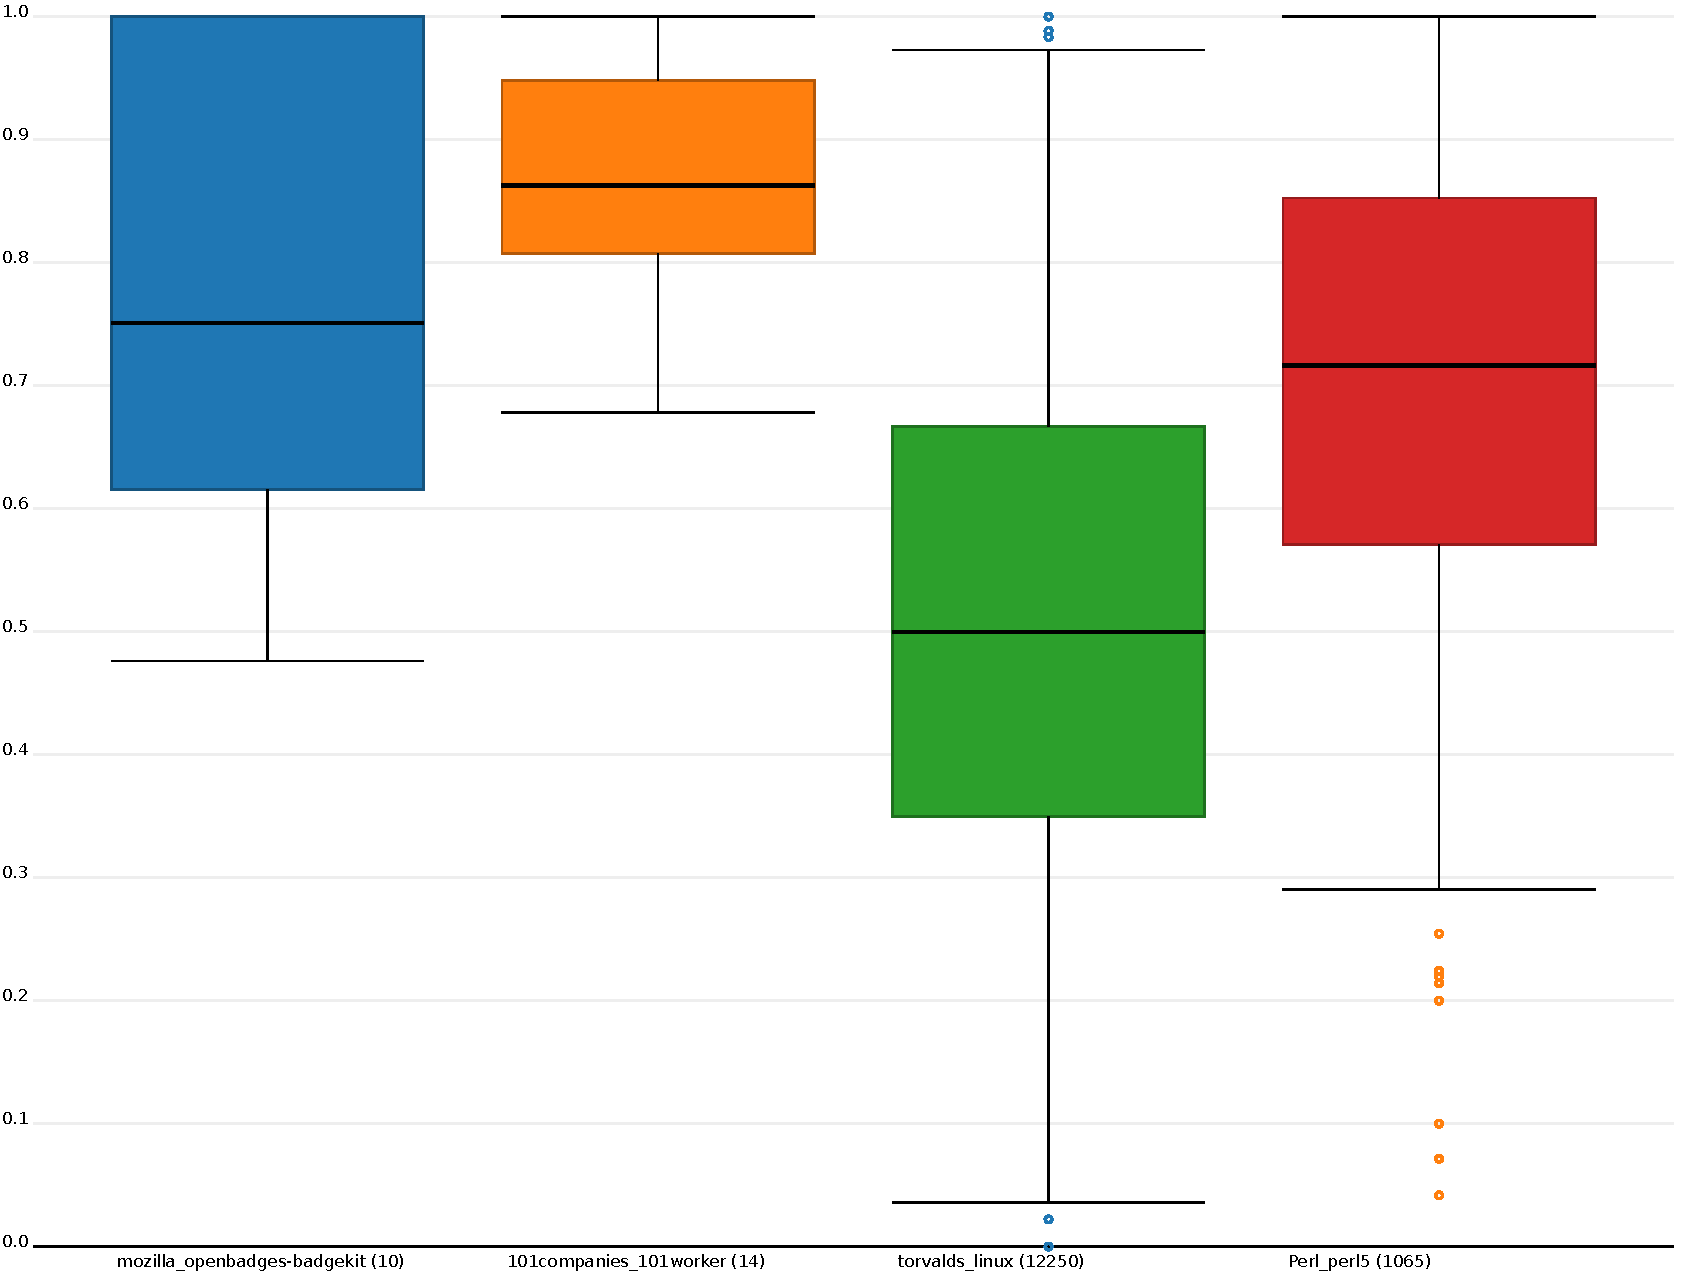
\includegraphics[width=0.8\textwidth]{img/subject_limit.pdf}
    \caption{Subject Limit Boxplot}
    \label{fig:bp_subject_limit}
\end{figure}

Figure \ref{fig:bp_subject_limit} shows the repository-level boxplots for the subject limit criterion for all 4 repositories. The number behind the labels denotes the number of authors that were evaluated in the graph. Surprisingly, the linux kernel has the worst results, followed by the badgekit and the perl5 and then the 101worker with the best results.

\begin{figure}[p]
    \centering
    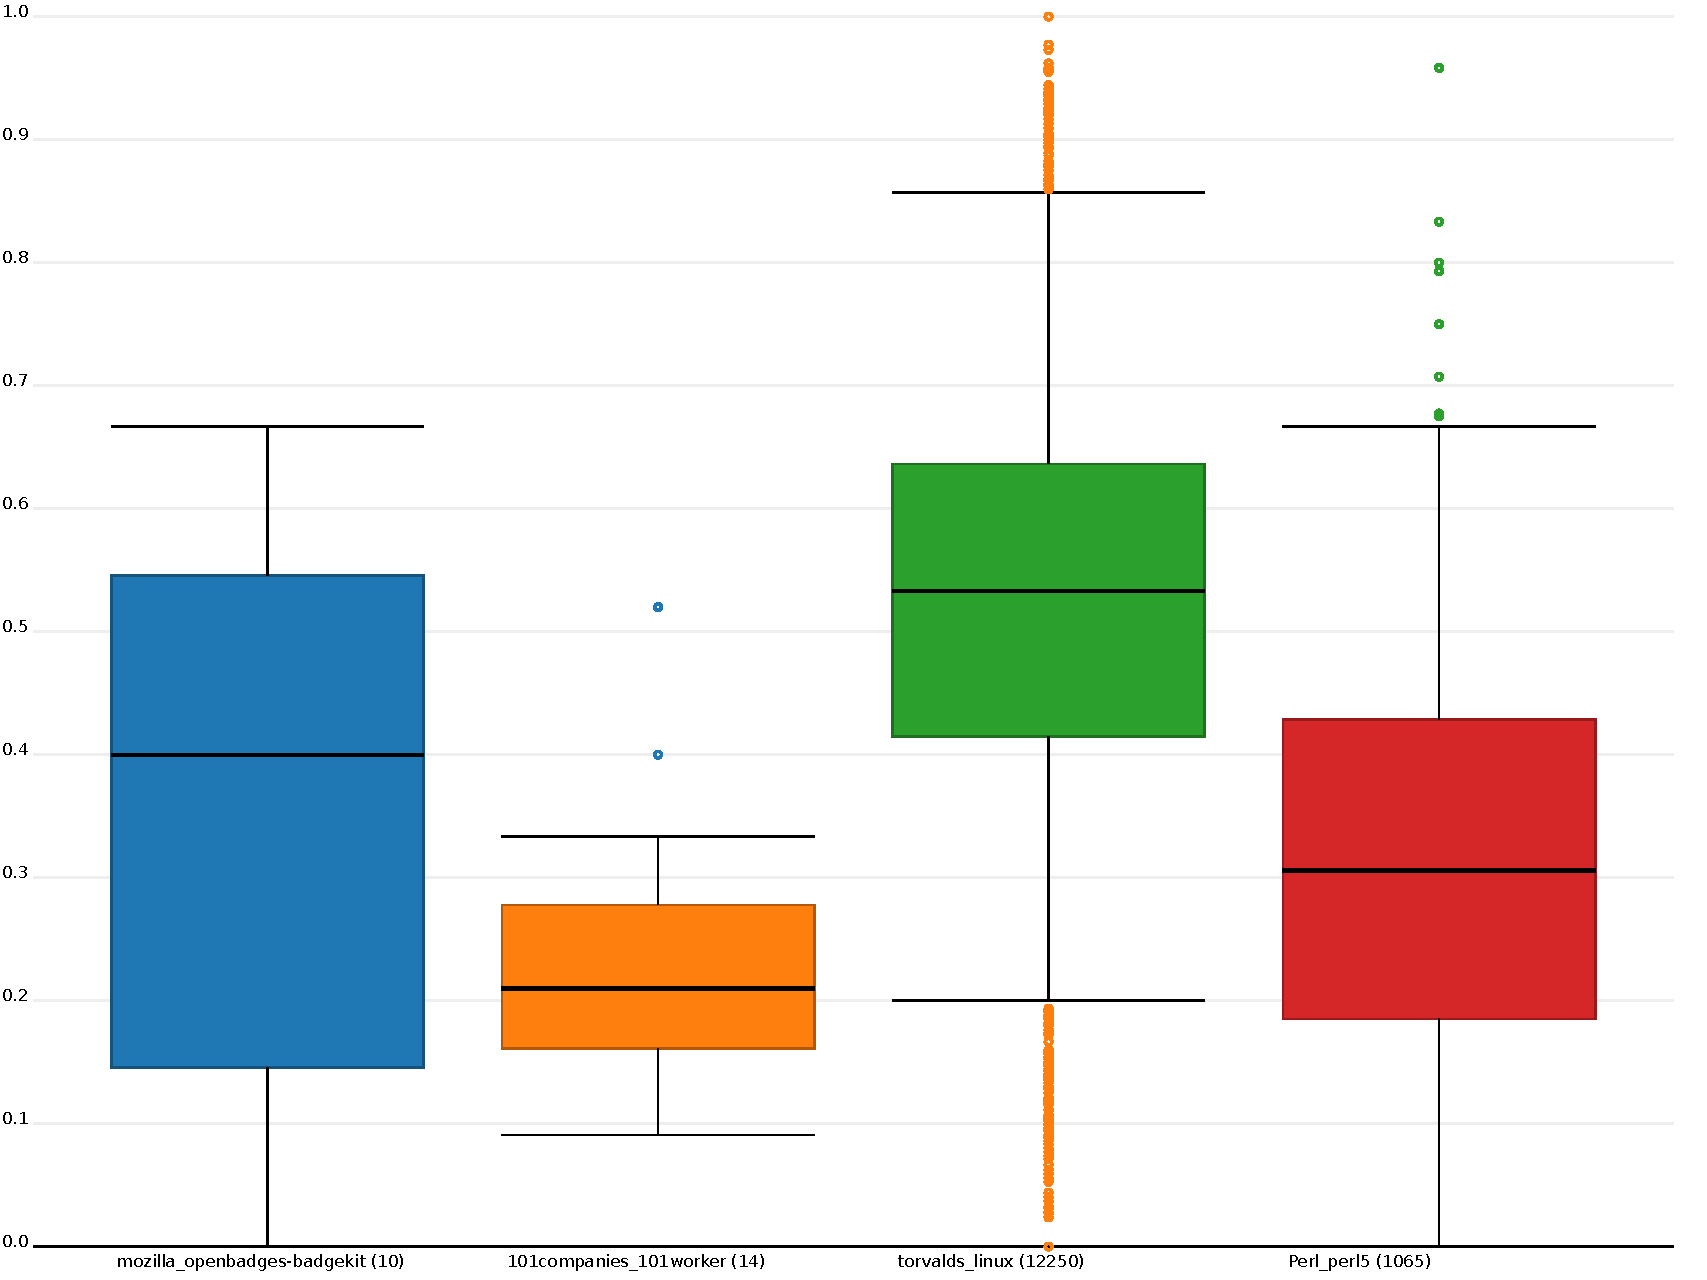
\includegraphics[width=0.8\textwidth]{img/imperative_subject.pdf}
    \caption{Imperative Subject Boxplot}
    \label{fig:bp_imperative_subject}
\end{figure}

\begin{figure}[p]
    \centering
    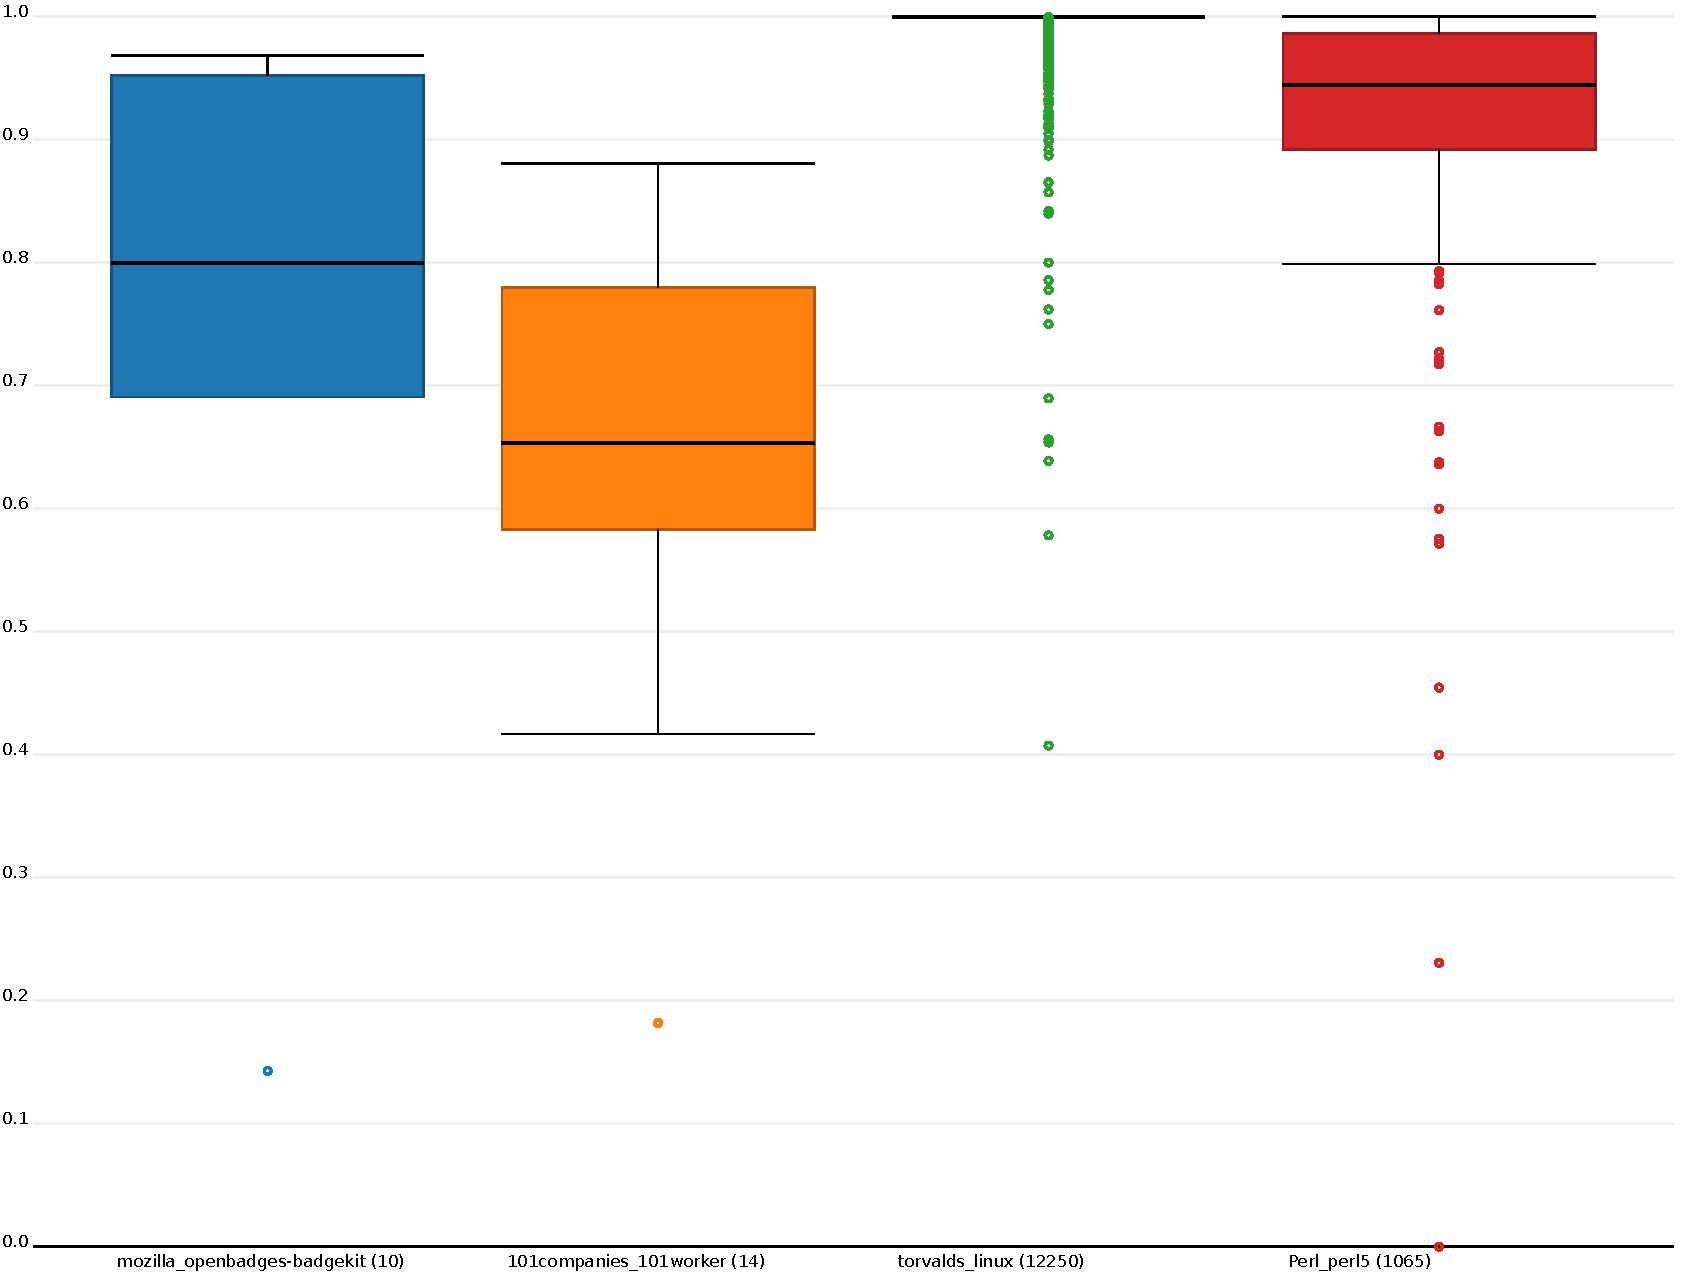
\includegraphics[width=0.8\textwidth]{img/no_short_message.pdf}
    \caption{No Short Message Boxplot}
    \label{fig:bp_no_short_message}
\end{figure}

On the other hand, figure \ref{fig:bp_imperative_subject} shows that authors of the linux kernel use the imperative mood for the subject the most, while the authors of the 101worker rarely do. Additionally, figure \ref{fig:bp_no_short_message} shows that linux kernel authors do not write short commit messages, while the authors of the 101worker do. This observation coincides with our estimations for the worker, since that criterion was inspired by a prevalence for 1-word commits in that repo.

\begin{figure}[p]
    \centering
    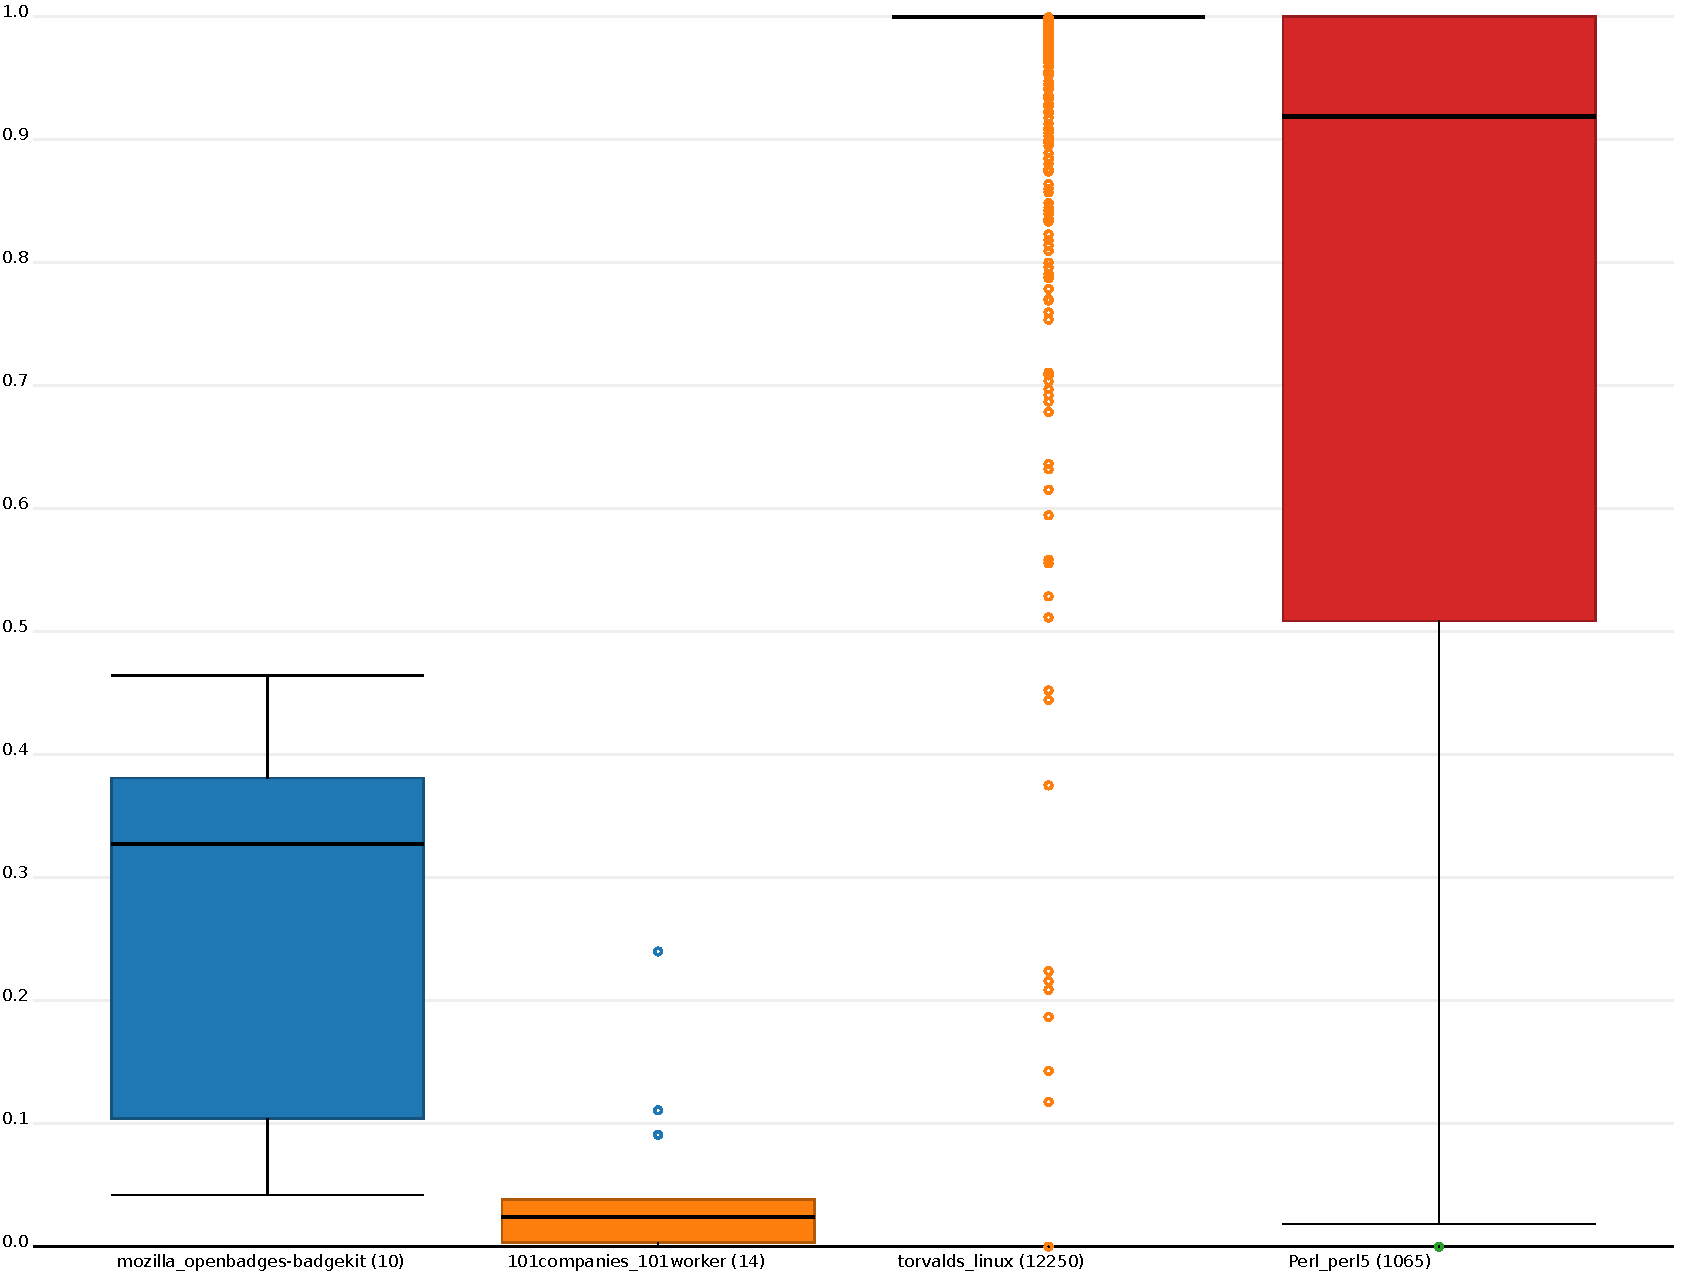
\includegraphics[width=0.8\textwidth]{img/body_used.pdf}
    \caption{Body Used Boxplot}
    \label{fig:bp_body_used}
\end{figure}

One significant difference between the two small repos (badgekit and 101worker) and the big repos (perl and linux kernel) stands out in figure \ref{fig:bp_body_used}. The big repos both make heavy use of the body, while it is almost never used by the worker and only sometimes by the badgekit.

\begin{figure}[p]
    \centering
    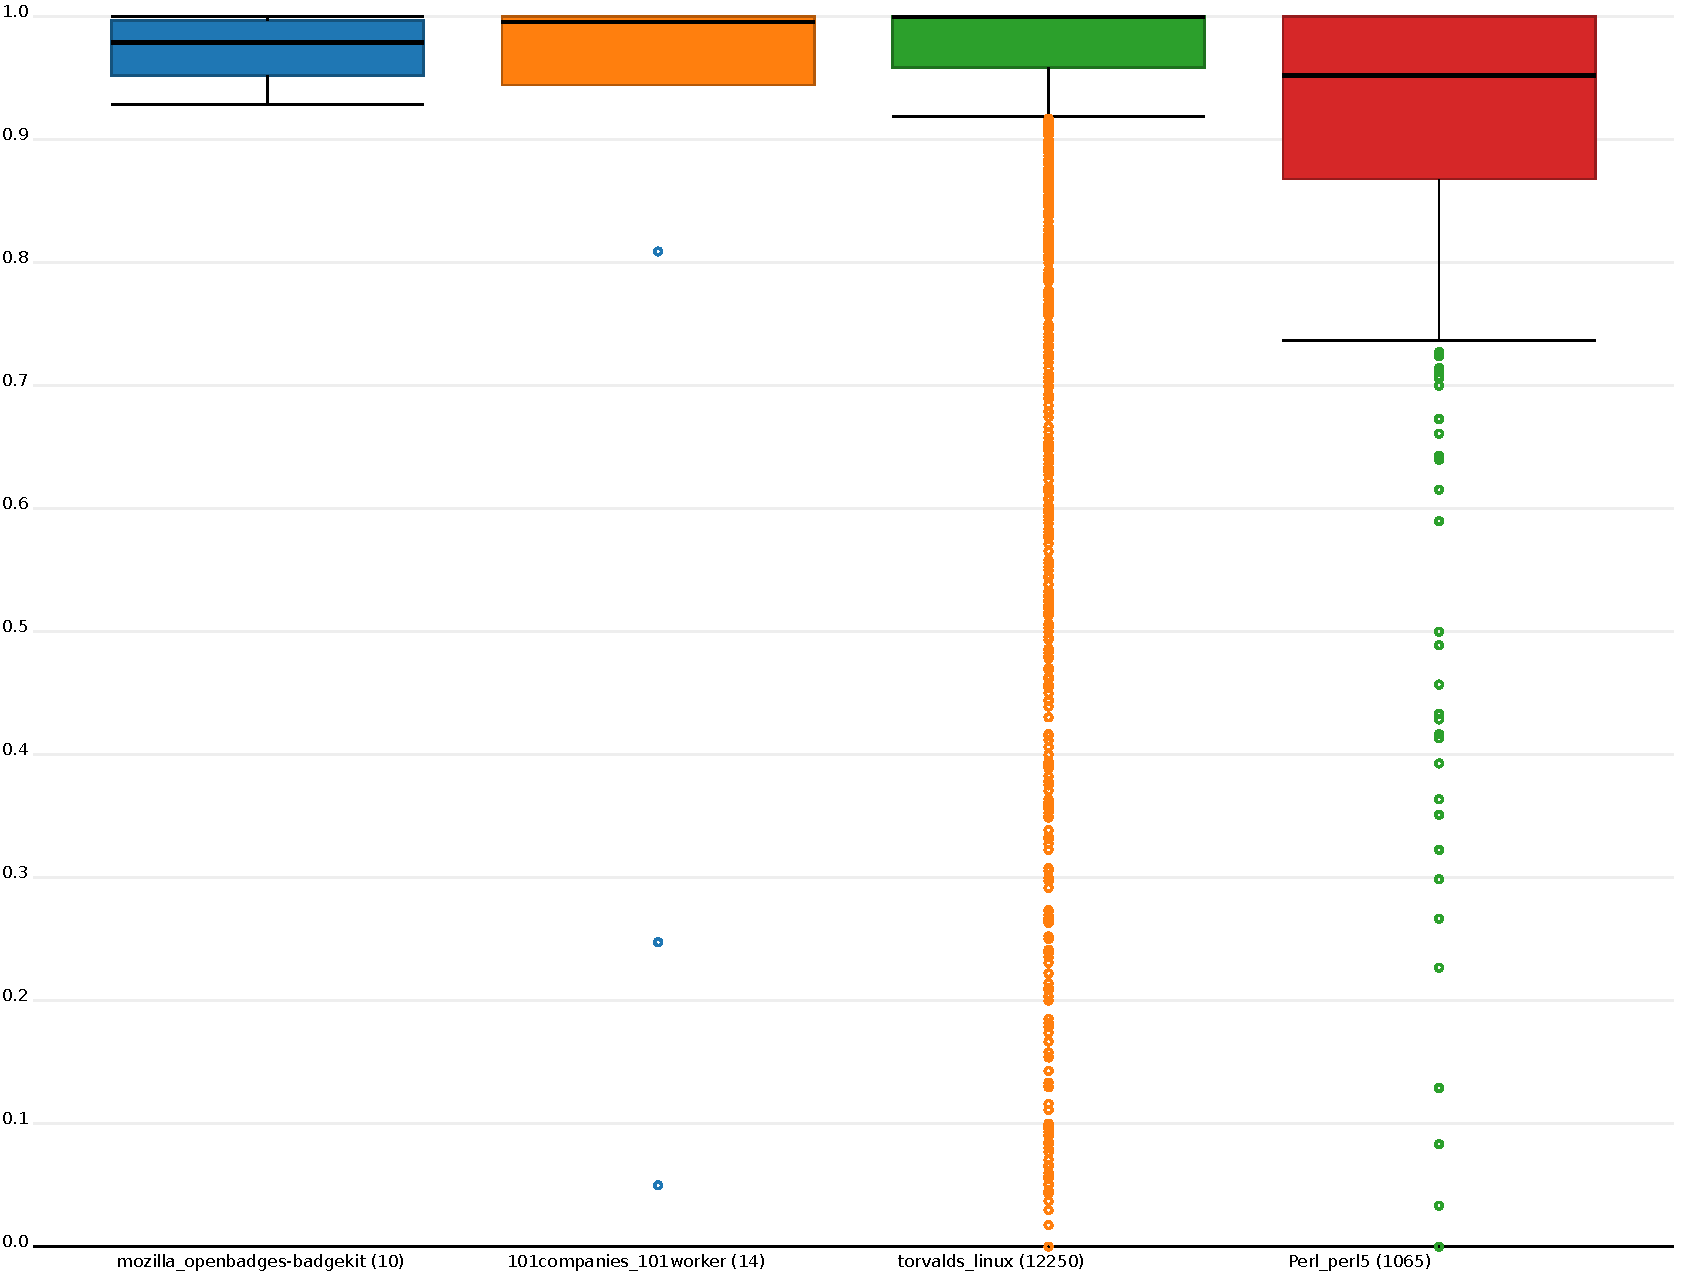
\includegraphics[width=0.8\textwidth]{img/no_period_subject.pdf}
    \caption{No Period Subject Boxplot}
    \label{fig:bp_no_period_subject}
\end{figure}

Finally, figure \ref{fig:bp_no_period_subject} shows that generally none of the repositories put a period at the end of the subject line. This means, that this criterion could be disregarded, if similar behaviour can be observed in other repositories.

The boxplots for the other criteria are available in our Git and were not included here in order to save space.

Based on these results, it is surprisingly hard to draw justified conclusions and answer our first research question positively. While the linux kernel is certainly the most high-profile Git repository in our selection and one might expect a high commit quality from the contributing authors, considering the median it is outperformed in four of thirteen criteria by the other repositories.

Since we lack further objective judgements on the ``goodnes'' of commits or repositories, we can not evaluate if meeting our criteria means having ``good'' commits.

On the other hand, it can be argued that meeting the seven official criteria means having good commits \emph{per definition}, since they have been taken from the official guidelines, and are therefore themselves the missing objective judgement.

In summary, while the analysis results are certainly interesting to look at, they offer no unambiguous answer to our first research question.

\subsection{Machine Learning}
\label{sec:results2}


%\noindent
%Summarize results in terms of tables, charts, and other kinds of
%figures.
%
%Explain and interpret the results.
%
%Get back to the research question and make sure that it is explicitly answered.
